%% Presented at Videnskabhistorisk Selskab, København

\documentclass[fleqn]{beamer}
\usetheme{metropolis}
\usepackage[utf8]{inputenc}
\usepackage[T1]{fontenc}
\usepackage{amsmath, amssymb}
\usepackage{graphicx}
\usepackage{hyperref}
\usepackage{amsfonts}
\usepackage{tikz-cd}
\usepackage{array}
\usepackage{adjustbox}



\usepackage{tikz}
\usetikzlibrary{arrows.meta, positioning, shapes.geometric, calc,
  decorations.markings, decorations.pathreplacing,
  decorations.pathmorphing}

% A TikZ style for curved arrows of a fixed height, due to AndréC.
\tikzset{curve/.style={settings={#1},to path={(\tikztostart)
    .. controls ($(\tikztostart)!\pv{pos}!(\tikztotarget)!\pv{height}!270:(\tikztotarget)$)
    and ($(\tikztostart)!1-\pv{pos}!(\tikztotarget)!\pv{height}!270:(\tikztotarget)$)
    .. (\tikztotarget)\tikztonodes}},
    settings/.code={\tikzset{quiver/.cd,#1}
        \def\pv##1{\pgfkeysvalueof{/tikz/quiver/##1}}},
    quiver/.cd,pos/.initial=0.35,height/.initial=0}

\title{Niels Bohr's Philosophical Background}
\subtitle{}
\author{Hans Halvorson}
\institute{Princeton University}
\date{April 22, 2025}

\usepackage[style=authoryear, backend=biber, natbib=true, doi=true]{biblatex} % Chicago style with Biber backend
\addbibresource{phil19.bib}
\addbibresource{~/research/grundriss.bib}

\begin{document}

\begin{frame}
   \titlepage
\end{frame}

\section{Introduction}

\begin{frame}{Audience and Speaker}

  \begin{itemize}
  \item I am not (really) a historian of science.
  \item My job description is ``philosopher'', but I think it means
    ``hopelessly interdisciplinary''.
  \item My intended audience today is not \emph{fagfilosoffer}. It is
    primarily people who, like me, (a) care about the ``meaning'' of
    physics, and (b) are confused about the current moment in the
    history of physics.
  \end{itemize}

\end{frame}

\begin{frame}{The current moment in physics}

  \begin{tikzpicture}[remember picture, overlay]
    % Place Kierkegaard image
    \node[anchor=south west] (kierkegaard) at (8,0) 
      {\includegraphics[width=1cm]{kierkegaard.jpg}};
  \end{tikzpicture}

  \begin{enumerate}
  \item Students of physics cannot
    \emph{\textbf{\textcolor{blue}{tilegne}}\tikz[remember
      picture,baseline] \coordinate (tilegne); } quantum mechanics
    \begin{itemize}
    \item ``Shut up and calculate''
    \item ``Bohr solved the foundational crisis in physics''
    \item ``Philosophy is dead''
    \end{itemize}
  \item Students of physics defect to philosophy
  \end{enumerate}

\begin{tikzpicture}[remember picture, overlay]
  \draw[->, thick]
    (kierkegaard.south west)
    to[out=225, in=90] ([yshift=0.6em]tilegne);
\end{tikzpicture}
  


\end{frame}

\begin{frame}{My attempt to get unconfused}

  \begin{itemize}
  \item Bring to bear all the tools of understanding we have:
    mathematical, conceptual, historical
  \item Earlier career: I focused on mathematical clarification
  \item More recently: I have focused on understanding Bohr's thought
    --- which led me to language, culture, and the history of (Danish)
    philosophy
    \begin{itemize}
    \item Why Bohr and not just the history of quantum physics
      generally?
    \end{itemize}
  \end{itemize}

\end{frame}

\begin{frame}{Why \emph{philosophical} background?}

  {\Huge Philosophy as \emph{Livsanskuelse} }



\end{frame}

\section{Bohr's philosophy}

\begin{frame}{Objective Description}
  
  ``No man who is called a philosopher really understands what one
  means by the complementary description. \dots They did not see that
  it was an objective description, and that it was the only possible
  objective description.'' (Interview with T. Kuhn, Nov 17, 1962)

\end{frame}

\begin{frame}{\mbox{}}

  ``The notion of complementarity does not imply any renunciation of
  detailed analysis limiting the scope of our enquiry, but simply
  stresses the character of objective description, independent of
  subjective judgment, in any field of experience where unambiguous
  communication essentially involves regard to the circumstances in
  which evidence is obtained. In logical respect, such a situation is
  well known from discussions about psychological and social problems
  where many words have been used in a complementary manner since the
  very origin of language.'' \citep[1105]{rutherford}


\nocite{koch2016danske}

\end{frame}




\begin{frame}{\mbox{}}

  ``Far from indicating a departure from our position as detached
  observers, the notion of complementarity represents the logical
  expression for our situation as regards objective description in
  this field of experience, which has demanded a renewed revision of
  the foundation for the unambiguous use of our elementary concepts.''
  \citep[54]{unity55}


\end{frame}

\begin{frame}{\mbox{}}

  ``By the lesson regarding our position as observers of nature, which
  the development of physical science in the present century has given
  us, a new background has, however, been created just for the use of
  such words as objectivity and subjectivity. From a logical
  standpoint, we can by an objective description only understand a
  communication of experience to others by means of a language which
  does not admit ambiguity as regards the perception of such
  communications.'' \citep[386]{religion54}

\end{frame}


\begin{frame}{Subject and Object}

  ``\dots volition and causation are equally indispensable elements in
  the relationship between subject and object, which is the most
  central problem of epistemology''

  \bigskip ``Samtidig drejer det sig på begge områder om
  idealisationer, hvis naturlige begrænsning kan gøres til genstand
  for undersøgelse og som betinger hinanden i den forstand, at
  viljesfølelse og årsagskrav er lige uundværlige elementer i
  forholdet mellem subjekt og objekt, som er erkendelsesproblemets
  kerne.'' \citep[82]{bohr-atomteori}

\end{frame}

\begin{frame}{Contemplation and Action}

  ``The complementary way in which words like contemplation and
  volition are used has especially to be taken into account when
  turning to the problem of the freedom of the will, discussed by
  philosophers through the ages.'' \citep[66]{unity}

\end{frame}




\section{The Philosophical Context}

\begin{frame}{Dialectical Progression to Absolute Knowledge}

\begin{center}
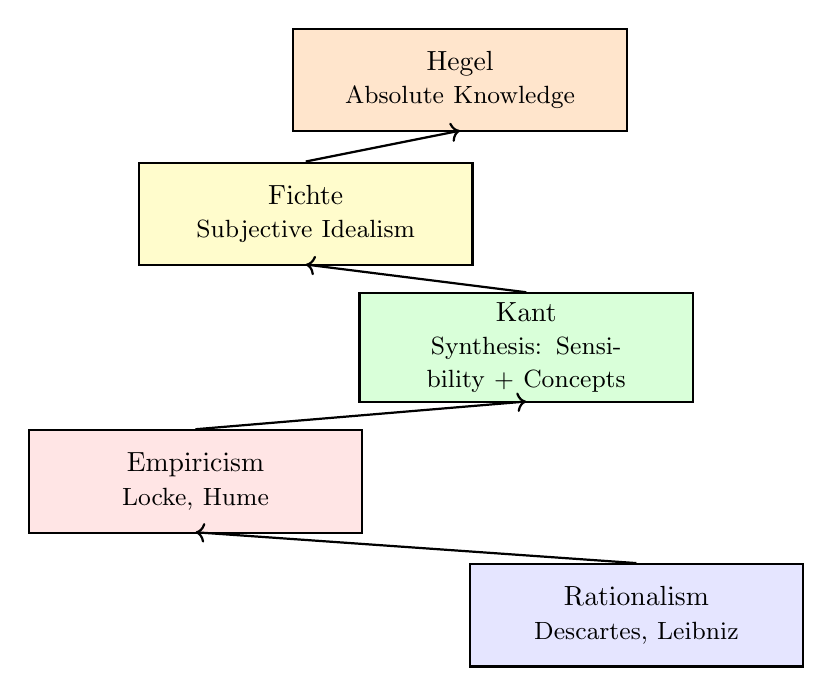
\begin{tikzpicture}[
  every node/.style={align=center},
  box/.style={rectangle, draw, thick, text width=4cm, minimum height=1.3cm},
  ->, thick
]

% Tighter spacing
\def\xstep{2.8}  % horizontal offset
\def\ystep{1.7}  % vertical spacing (box height)

% Nodes: zigzag positions, touching vertically
\node (rationalism) [box, fill=blue!10] at (2*\xstep, 0) 
  {Rationalism \\ \small Descartes, Leibniz};

\node (empiricism) [box, fill=red!10] at (0, \ystep) 
  {Empiricism \\ \small Locke, Hume};

\node (kant) [box, fill=green!15] at (1.5*\xstep, 2*\ystep) 
  {Kant \\ \small Synthesis: Sensibility + Concepts};

\node (fichte) [box, fill=yellow!20] at (0.5*\xstep, 3*\ystep) 
  {Fichte \\ \small Subjective Idealism};

\node (hegel) [box, fill=orange!20] at (1.2*\xstep, 4*\ystep) 
  {Hegel \\ \small Absolute Knowledge};

% Vertical arrows from each box's top to the bottom of the next
\draw[->] (rationalism.north) -- ($(empiricism.south)+(0,0.02)$);
\draw[->] (empiricism.north) -- ($(kant.south)+(0,0.02)$);
\draw[->] (kant.north) -- ($(fichte.south)+(0,0.02)$);
\draw[->] (fichte.north) -- ($(hegel.south)+(0,0.02)$);

\end{tikzpicture}
\end{center}  


\end{frame}


\begin{frame}{The Subject-Object Problem: From Kant to Hegel}

\begin{itemize}
\item \textbf{Kant}: Introduced the distinction between the knowing
  subject and the object of experience. The object is constituted
  through the subject's forms of intuition and categories.

\item \textbf{Fichte}: Radicalized Kant — all objectivity arises from
  the self-positing activity of the \emph{I}. The object is a
  projection of the subject’s own limitation.

\item \textbf{Hegel}: Resolved the opposition of subject and object
  through dialectic. The Absolute is the self-unfolding unity of
  subject and object in Spirit (\emph{Geist}).

\end{itemize}  

\end{frame}

\begin{frame}{Hegel}

  ``It is thus `the absolute method of knowing,' a spiritual
  excitation that is the immanent development of the concept. When the
  concept is fully revealed, the recipient of that revelation (i.e.,
  Hegel) has overcome the split between subject and object. The
  history of philosophy is complete and the absolute is present within
  human time. Being and thinking are the same.'' \citep[35]{rosen}

\end{frame}

\begin{frame}{Kierkegaard on Hegel}

  ``Hegelian philosophy culminates in the thesis that the outer is the
  inner and the inner is the outer.'' \newline \emph{Concluding
    Unscientific Postscript}

\end{frame}

\begin{frame}{Kierkegaard on Hegel}

  ``So we return to the two paths of reflection, and have not
  forgotten that it is an existing spirit that poses the question,
  quite simply a human being. Nor can we forget that his existing is
  just what will stop him going both ways at once, while his anxious
  question will prevent him from frivolously and fantastically
  becoming subject-object. Which of these two paths, then, is the path
  of truth for an existing spirit? For only the fantastic I-I is
  finished with both paths all at once, or proceeds methodically down
  both paths simultaneously, a gait so inhuman for an existing human
  that I do not risk recommending it.'' (Postscript, Hannay
  translation, p 162)

\end{frame}

\begin{frame}{Complementarity between reflection (overvejelse) and
    decision (afgørelse)}

  ``Once subjectivity is taken away, and passion from subjectivity,
  and infinite interest from passion, there is absolutely no decision
  [afgørelse] at all, on this problem or any other. All decision, all
  essential decision, lies in subjectivity. At no point does an
  observer (and that is what objective subjectivity is) have any
  infinite need of a decision, and at no point sees it.'' (Postscript,
  p 29)

\end{frame}

\section{Danish philosophy}


\begin{frame}{Philosophical Background to Niels Bohr}

\begin{center}
\begin{tikzpicture}[every node/.style={align=center}, xscale=1, yscale=1]

% Dimensions
\def\imgw{2.5cm}
\def\imgh{3cm}
\def\xgap{3.5}
\def\ygap{4}

% Top row
\node (holberg) at (0,0) 
  {\includegraphics[width=\imgw,height=\imgh]{holberg.jpg} \\ \small Ludvig Holberg};

\node (sibbern) at (\xgap,0) 
  {\includegraphics[width=\imgw,height=\imgh]{sibbern.jpg} \\ \small Frederik Sibbern};

\node (moeller) at (2*\xgap,0) 
  {\includegraphics[width=\imgw,height=\imgh]{moller.jpg} \\ \small Poul Møller};

% Bottom row
\node (kierkegaard) at (0,-\ygap) 
  {\includegraphics[width=\imgw,height=\imgh]{kierkegaard.jpg} \\ \small Søren Kierkegaard};

\node (nielsen) at (\xgap,-\ygap) 
  {\includegraphics[width=\imgw,height=\imgh]{nielsen.jpg} \\ \small Rasmus Nielsen};

\node (hoffding) at (2*\xgap,-\ygap) 
  {\includegraphics[width=\imgw,height=\imgh]{hoffding.jpg} \\ \small \textbf{Harald Høffding}};

\end{tikzpicture}
\end{center}  


\end{frame}

\begin{frame}{Ludvig Holberg: Tone Setter for Danish Philosophy}

\begin{columns}
  \begin{column}{0.4\textwidth}
    \includegraphics[width=\linewidth]{holberg.jpg}  % Replace with actual image path

    \vspace{0.5em}
    \centering
    {\small\textit{Ludvig Holberg (1684–1754)}\\
    Playwright, historian, philosopher}
  \end{column}

  \begin{column}{0.6\textwidth}
    \begin{itemize}
      \item Advocated for clarity, reason, and practical civic values.
      \item Blended satire and empiricism to challenge intellectual pretension.
      \item Strongly opposed scholasticism — especially abstract metaphysics and theological hairsplitting.
      \item Promoted a philosophy grounded in common sense and historical learning.
      \item Set the tone for a distinctly Danish style of thought: moderate, worldly, ironic.
    \end{itemize}
  \end{column}
\end{columns}

\end{frame}

\begin{frame}{Danish philosophy}

  ``Danish thinking has been most interested in
  \underline{psychological} and \underline{ethical} questions, and it
  has usually been critical of the practice of system-building.''
  \citep[2]{hoffding1909}


\end{frame}

\begin{frame}{Sibbern on Hegel}

  \includegraphics[scale=0.4]{hegels-philosophie.pdf}

\end{frame}

\begin{frame}{Bohr on Møller}

  ``Nor do I need bring to mind the amusing story about the licentiate
  in \emph{The Adventures of a Danish Student}, which I related at my
  talk in Pasadena to elucidate the complementary use of terminology
  in psychology. The point here is, of course, that even though every
  unambiguous communication requires distinction between a subject and
  an object, the subject implied in a given situation can wholly or
  partially be included in the objective content of a communication
  about another situation.''

  \medskip NB to Delbr{\"u}ck, July 25, 1959

\end{frame}


\begin{frame}{Sibbern and Møller: Resistance to Hegelianism}

\begin{columns}
  \begin{column}{0.45\textwidth}
    \begin{tabular}[t]{@{}m{1.7cm} m{2.5cm}@{}}
      \includegraphics[height=1.7cm]{sibbern.jpg} & 
      \begin{minipage}[t]{\linewidth}
        \vspace{0pt}
        \small \textit{Frederik Sibbern} \\[-0.3em]
        \small (1785–1872)
      \end{minipage}
    \end{tabular}
  \end{column}

  \begin{column}{0.45\textwidth}
    \begin{tabular}[t]{@{}m{1.7cm} m{2.5cm}@{}}
      \includegraphics[height=1.7cm]{moller.jpg} & 
      \begin{minipage}[t]{\linewidth}
        \vspace{0pt}
        \small \textit{Poul Møller} \\[-0.3em]
        \small (1794–1838)
      \end{minipage}
    \end{tabular}
  \end{column}
\end{columns}
  
  
\begin{itemize}
\item Both Sibbern and Møller engaged critically with Hegel’s
  philosophy — especially its abstract systematization and speculative
  ambitions.
\item Sibbern emphasized lived experience, emotional life, and
  psychological observation over metaphysical constructs.
\item Møller responded with irony and literary sensibility, expressing
  skepticism toward philosophical totality.
\item Their opposition set the stage for Kierkegaard's more radical
  critique of Hegelianism — but in a tone that remained
  characteristically Danish: modest, ironic, and anti-systematic.
\end{itemize}

\end{frame}

\begin{frame}{\mbox{}}

\Huge The missing link? 


\end{frame}


\begin{frame}{Hypothesis}

  Rasmus Nielsen transformed the qualitative epistemological and
  psychological ideas of Sibbern, Møller, Kierkegaard, etc.\ into
  something that was scientifically useful for Bohr.

  \vspace{2em}

\adjustbox{scale=0.8,center}{%
\begin{tikzcd}[ampersand replacement = \&]
  \&\&\&\& \text{H. Høffding} \\
  \text{S. Kierkegaard} \&\& \text{R. Nielsen} \&\&\&\& \text{N. Bohr} \\
  \&\&\&\& \text{Ch. Bohr} \arrow[from=2-1, to=2-3] \arrow[from=2-3,
  to=1-5] \arrow[from=2-3, to=3-5] \arrow[from=1-5, to=2-7]
  \arrow[from=3-5, to=2-7]
\end{tikzcd}
}

\end{frame}

\begin{frame}{Preparing the ground for Bohr}

\begin{tikzcd}[ampersand replacement=\&]
	\& {\text{Sibbern}} \& {\text{M{\o}ller}} \\
	\\
	{\text{Kierkegaard}} \&\& {\text{Nielsen}} \\
	\\
	{\text{Christian Bohr}} \&\& {\text{H{\o}ffding}} \\
	\\
	\\
	\&\& {\text{Niels Bohr}}
	\arrow[from=1-3, to=3-1] % Møller to Kierkegaard
	\arrow[from=1-3, to=3-3] % Møller to Nielsen
	\arrow[from=3-1, to=3-3] % Kierkegaard to Nielsen
	\arrow[from=1-2, to=3-1] % Sibbern to Kierkegaard
	\arrow[from=1-2, to=3-3] % Sibbern to Nielsen
	\arrow[from=3-1, to=5-3] % Kierkegaard to Høffding
	\arrow[from=3-3, to=5-3] % Nielsen to Høffding
	\arrow[from=3-3, to=5-1] % Nielsen to Christian Bohr
	\arrow[from=5-3, to=8-3] % Høffding to Niels Bohr
	\arrow[from=5-1, to=8-3] % Christian Bohr to Niels Bohr
	\arrow[curve={height=-30pt}, from=1-3, to=8-3] % Møller to Niels Bohr
\end{tikzcd}
  

\end{frame}


\begin{frame}{Rasmus Nielsen: The forgotten philosopher}

  ``At first it was Rasmus Nielsen, whose enthusiastic references to
  Kierkegaard and whose rousing eloquence had the greatest influence
  on me.'' \citep{hoffding1909}

  \vfill

  ``No one who studies the life of the mind in nineteenth-century
  Denmark, will be able to skip over [Nielsen's] great philosophical
  writings, and everyone who got to hear his lectures at the
  university will remember him as a great awakener and a rare
  personality.'' \citep{brandes1889}



\end{frame}

\begin{frame}{Nielsen against Hegel: No Absolute Knowledge}

  \begin{quote}
    ``Vi kunne derfor hverken i Naturen eller i Historien og
    ligesaalidt i Religionen selv vente at komme til absolut Viden, da
    det netop er denne Verdens ejendommelige Charakteer, at alle Livets
    Elementer i den adsplittes i løsrevne Brudstykker.''\\[0.5em]
    \hfill \citep{speculative1842}
  \end{quote}

  \vspace{1em}
  \begin{itemize}
    \item Hegel: Reality and knowledge form a unified totality.
    \item Nielsen: The world disaggregates into ``løse Brudstykker''
      --- no absolute synthesis is possible.
    \item \textbf{Bohr:} Echoes this view with his idea that physical
      phenomena must be described from mutually incompatible
      perspectives.
  \end{itemize}
\end{frame}

\begin{frame}{Nielsen's scientific turn}

  ``As my recent writings show, it has been my goal, for a number of
years, to clarify and demonstrate the relationship between philosophy
and the separate sciences as comprehensively as possible. The future
of philosophy depends in an essential way on a thorough understanding
and accurate determination of this relationship.'' \citep[18]{grund}
  
\end{frame}

\begin{frame}

\begin{figure}
  \centering \includegraphics[scale=0.5]{prop1.png}
\end{figure}
\end{frame}

\begin{frame}

\begin{figure}
\centering
\includegraphics[scale=0.65]{prop2.jpg}
\end{figure}
\end{frame}

\begin{frame}

\begin{figure}
\centering
\includegraphics[scale=0.5]{prop3.jpg}

\end{figure}
\end{frame}





\begin{frame}{Nielsen and Høffding: Objectivity Without Absolutes}

\begin{itemize}
  \item \textbf{Rasmus Nielsen}: Proposed a \textbf{law of objectivization}:
    \begin{quote}
      There is no object without a corresponding objectification — and
      no objectification without an objectifying subject.
    \end{quote}
    Reality is not given independently, but always mediated by the
    activity of a subject.

  \item \textbf{Harald Høffding}: Extended Nielsen’s insight. Claimed that:
    \begin{quote}
      There is no final or absolute objectifying subject.
    \end{quote}
    Subjectivity itself is historically and psychologically
    conditioned — there is no Archimedean point. Objectivity emerges
    from an evolving network of perspectives.
\end{itemize}

\end{frame}



\begin{frame}{Objectiveringslov}

  ``No object without a corresponding objectification; it is an a
  priori law that underwrites all empiricism, a basic law that in
  science is, if possible, even more unshakable than Newton's law of
  gravity. From this it can be seen, that a critical boundary, a
  boundary line, on whose one side we have the objectivizing
  subjectivity, while the object is standing on the other side, is
  confused and meaningless.'' \citep[41]{avg}

\end{frame}




\begin{frame}{Rasmus Nielsen: The Law of Objectification}
  \textbf{Central Thesis:} There is no object without an objectifying subject.

  \vspace{1em}
  \begin{itemize}
    \item Nielsen’s \emph{law of objectification} (\textit{Objectiveringsloven}) states that 
    only what is objectified becomes an object.
    \item The subject plays an active, constitutive role in experience: objectivity is not merely \emph{given} but \emph{formed}.
    \item \textbf{Implication for Bohr:} The epistemological conditions for describing phenomena 
    may already embed subject-object relations, anticipating Bohr’s focus on measurement contexts.
  \end{itemize}

  \vspace{1em}
  \textit{“All objective relation is grounded in subjective reflection; this is a law of objectification, as strict as any natural law.”}
\end{frame}

\begin{frame}{\mbox{}}

  ``\dots all search for an ultimate subject is at variance with the
  aim of objective description which demands the contraposition of
  subject and object.''  \citep[]{unity}

  \vfill ``Nielsen believed that, to describe the interrelation
  between the subjective and the objective, an infinite analysis was
  needed, since every subject presupposes an object, and every object
  in turn a subject.''  \citep[189]{hoffding1909}

  \nocite{prop60}

\end{frame}


\begin{frame}{Mechanism vs.\ Teleology}
  \textbf{Nielsen's Dialectic:} Nature is governed both by mechanism (\textit{Andethed}) and teleology (\textit{Selvhed}).

  \vspace{1em}
  \begin{itemize}
    \item Nielsen critiques both reductionist mechanism \textit{and} vitalist teleology.
    \item He affirms that physical processes obey mechanistic laws \textit{but} life reflects inner purpose.
    \item Nature’s intelligibility, for Nielsen, requires both explanatory frames.
    \item \textbf{Connection to Bohr:} Bohr's complementarity likewise resists reduction---physics must account for wave and particle, description and limitation.
  \end{itemize}

  \vspace{1em}
  \textit{``The law of otherness is the law of matter; the law of selfhood is the law of life.''}
\end{frame}

\begin{frame}{Freedom and Necessity}
  \textbf{A Fundamental Tension:} Nielsen roots the contrast between
  scientific and ethical domains in a deeper metaphysical duality.

  \vspace{1em}
  \begin{itemize}
    \item Physical necessity arises from the law of \textit{Andethed}
      --- the logic of things governed by external relations.
    \item Freedom is grounded in \textit{Selvhed} --- the inner form of the self.
    \item \textbf{No sharp boundary:} The duality pervades all of reality, not just human action.
    \item \textbf{Relevance for Bohr:} Suggests a metaphysical precedent for Bohr’s openness to indeterminacy and contextual constraint.
  \end{itemize}

  \vspace{1em}
  \textit{``The struggle between freedom and necessity begins with life itself.''}
\end{frame}


\subsection{Harald Høffding}

\begin{frame}{\mbox{}}

  ``Just as form and content are abstractions, since in every act of
  cognition we have a combination of them, so it is with subject and
  object.''

  \bigskip ``Ligesom Emne og Form ere Abstraktioner, da vi i enhver
  Erkendelsesakt have en Forbindelse af dem, saaledes forholder det
  sig ogsaa med Subjekt og Objekt.'' \citep[297]{hoffding1910}

   \nocite{hoffding1909}

\end{frame}


\begin{frame}{\mbox{}}

  ``We could make our own subject an object for us, just as when we
  study it psychologically, e.g. to find out the forms by which it
  works in its cognition. These forms, which are systematized in the
  study of the categories of cognition, must be taken as facts. They
  are made subjects when reflection is applied to them. Every
  cognition takes place from a certain point of view, which it can be
  meaningful to ascertain [konstatere]. We then objectify the
  subject.'' \citep{hoffding1910}


\end{frame}

\begin{frame}{\mbox{}}

  ``When we consider something as an object, we must indicate the
  nature of the subject in relation to which it exists. And when we
  consider something as a subject, we must partly seek the objective
  context that determines its nature and thereby the contents and
  forms that are at its disposal, and on the other hand we need to
  note that by this investigation we ourselves make that subject into
  an object (if it is ourselves, then for ourselves in a somewhat
  different state, at any rate at a different moment, than before). We
  never have a pure subject ($S$), but always an objectively
  determined or yet an objectified subject ($S_o$). And we never have
  a pure object ($O$), but always a subjectivized object ($O_s$). $S$
  and $O$ are mere abstractions. What we have before us is always
  $S_o$ and $O_s$.'' \citep[298]{hoffding1910}


\end{frame}

\begin{frame}{\mbox{}}

  ``The act of becoming self-conscious, of making one's I (one's
  conditions, one's work, one's circumstances) into an object for
  itself, can always be repeated. The I that becomes self-conscious
  can itself become the object of a new act of self-consciousness, and
  so on. Such a series $(S_1 \prec S_2 \prec S_3 \prec S_4 \dots )$
  has already been mentioned above in connection with the possibility
  of an epistemological investigation into epistemology.''
  \citep[36]{hoffding1917}

\end{frame}

\begin{frame}{\mbox{}}

  ``Den Akt at blive sig selv bevidst, gøre sit Jeg (sine Tilstande,
  sit Arbejde, sine Kaar) til Genstand for sig, kan formelt stadig
  gentages. Det Jeg, der bliver sig selv bevidst, kan selv blive
  Genstand for en ny Selvbevidsthedsakt, og saaledes fremdeles. En
  saadan Række $(S_1 \{ S_2 \{ S_3 \{ S4 ....)$ er allerede omtalt
  ovenfor i Anledning af Muligheden af en erkendelsesteoretisk
  Prøvelse af Erkendelsesteorien.'' \citep[36]{hoffding1917}

\end{frame}

\section{Conclusion}

\begin{frame}{Summary}

  \begin{itemize}
  \item Bohr faced scientific challenges of great complexity and
    delicacy.
    \begin{itemize}
    \item Stability of matter
    \item The quantum of action
    \item Heisenberg and Schr{\"o}dinger
    \item Objective description
    \end{itemize}
  \item Bohr was fortunately equipped with a dynamic \emph{livssyn}
    that allowed him to take satisfaction in meeting challenges
    without final resolution.
  \end{itemize}

\end{frame}

\begin{frame}{Summary}

  \begin{itemize}
  \item Bonus: Significant figures (especially Sibbern and Nielsen)
    have been neglected
  \item Challenges:
    \begin{itemize}
    \item Bohr is both Danish and international
    \item Bohr is both scientist and humanist
    \end{itemize}
  \end{itemize}



\end{frame}




\section{References}

\begin{frame}[allowframebreaks]{References}

\printbibliography[heading=none]

\end{frame}





\end{document}



%%% Local Variables:
%%% mode: latex
%%% TeX-master: t
%%% End:
